\documentclass{article}
\usepackage{tikz}
\usepackage{verbatim} %commenting package
\usetikzlibrary{arrows}
\usetikzlibrary{calc,intersections,through,backgrounds}
\usetikzlibrary{automata}
\pagestyle{empty}
\begin{document}


% Define style for nodes
\tikzstyle{every node}=[circle, draw, fill=black,
                        inner sep=0pt, minimum width=4pt]

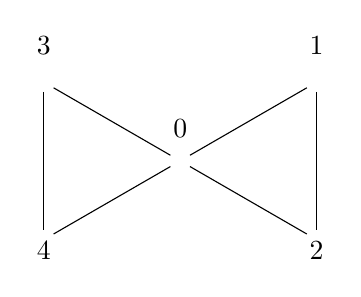
\begin{tikzpicture}
                        
\node[label={[shift={(0,0.1)}]1}](v1) at (30:2) {};

\node[label={[shift={(0,-0.5)}]2}](v2) at (-30:2) {};

\node[label={[shift={(0,0.1)}]3}](v3) at (150:2) {};

\node[label={[shift={(0,-0.5)}]4}](v4) at (210:2) {};

\node[label={[shift={(0,0.05)}]0}](v5) at (0,0) {};

\foreach \from/\to in { v5/v1, v5/v2, v5/v3, v5/v4,v3/v4,v1/v2}
    \draw  (\from) -- (\to);


\end{tikzpicture}


\end{document} 